%
% tikztemplate.tex -- template for standalon tikz images
%
% (c) 2019 Prof Dr Andreas Müller, Hochschule Rapperswil
%
\documentclass[tikz]{standalone}
\usepackage{amsmath}
\usepackage{times}
\usepackage{txfonts}
\usepackage{pgfplots}
\usepackage{csvsimple}
\usetikzlibrary{arrows,intersections,math}
\begin{document}
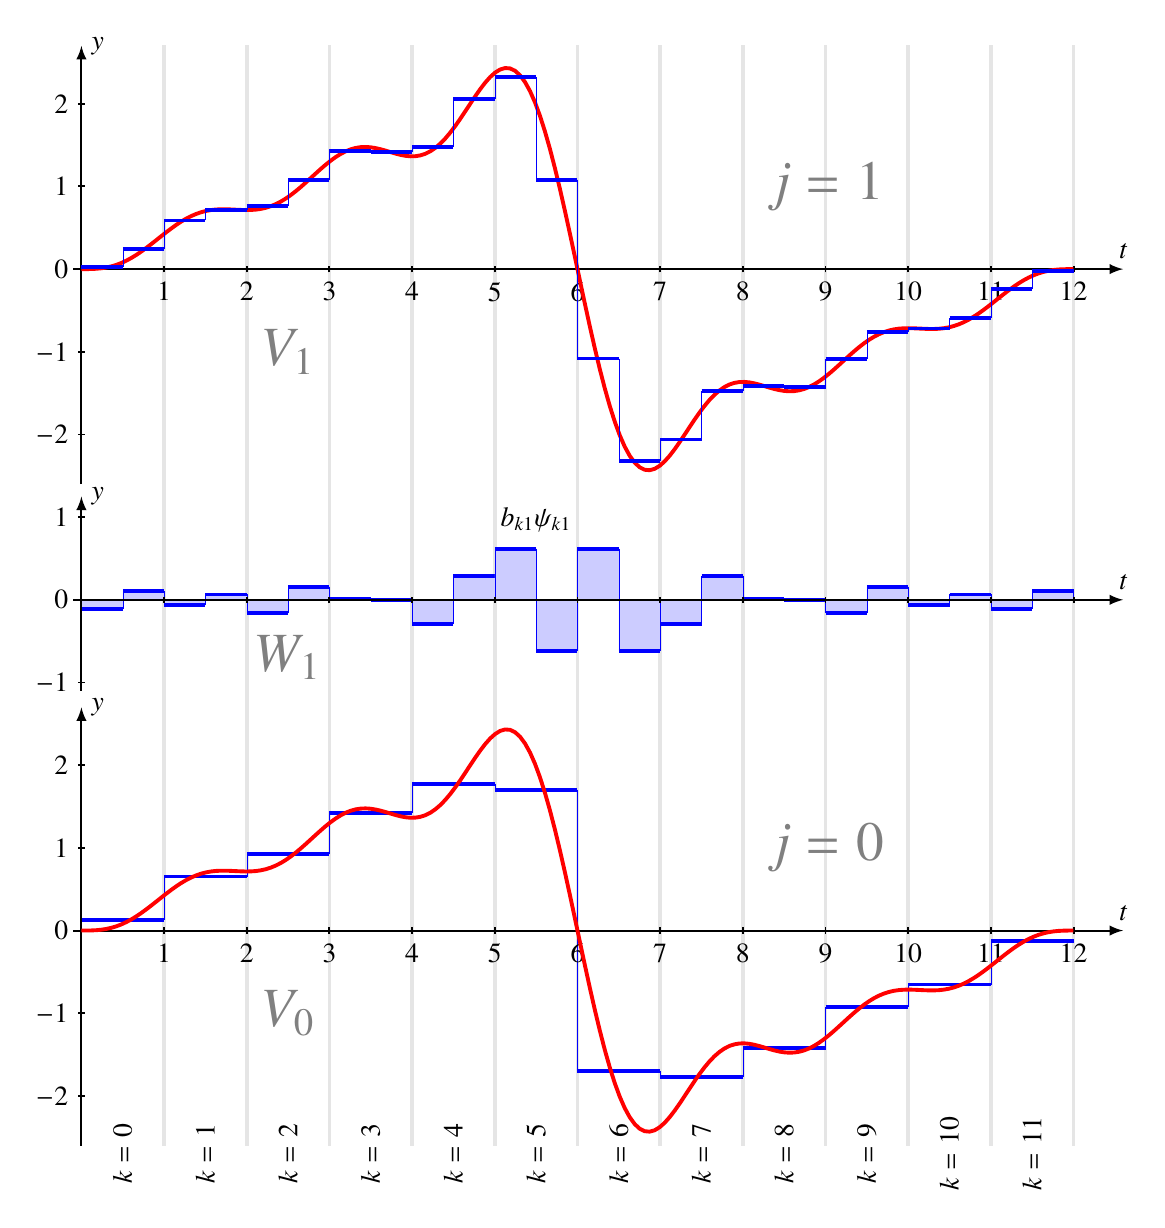
\begin{tikzpicture}[>=latex,scale=1.05]

\def\s{0.04}
\def\S{1}

\xdef\yold{0}

\begin{scope}
\clip (0.5,-2.6) rectangle (12.5,{8+2.7});
\foreach \x in {1,...,12}{
	\draw[line width=1.4pt,color=gray!20] (\x,-3)--(\x,13);
}
\end{scope}

%
% Approximation in Level 0
%
\foreach \x in {0,...,11}{

	\pgfmathparse{1.5*(-cos(30*(\x+\S))+cos(2*30*(\x+\S))/4-cos(3*30*(\x+\S))/9+cos(4*30*(\x+\S))/16-cos(5*30*(\x+\S))/25+cos(6*30*(\x+\S))/36+cos(30*(\x))-cos(2*30*(\x))/4+cos(3*30*(\x))/9-cos(4*30*(\x))/16+cos(5*30*(\x))/25-cos(6*30*(\x))/36)*6/3.14159}
	\xdef\y{\pgfmathresult}
	\draw[color=blue,line width=0.1pt] ({\x},{\yold})--({\x},{\y});
	\draw[color=blue,line width=1.4pt] ({\x},{\y})--({\x+\S},{\y});
	\xdef\yold{\y}
}

\draw[->,line width=0.7pt] (-0.1,0)--(12.6,0) coordinate[label={$t$}];
\draw[->,line width=0.7pt] (0,-2.6)--(0,2.7) coordinate[label={right:$y$}];
\foreach \x in {1,...,12}{
	\draw[line width=0.7pt] (\x,-\s)--(\x,\s);
	\node at (\x,-\s) [below] {$\x$};
}

\foreach \y in {-2,...,2}{
	\draw[line width=0.7pt] (-\s,\y)--(\s,\y);
	\node at (-\s,\y) [left] {$\y$};
}

\draw[line width=1.4pt,color=red]
	plot[domain=0:12,samples=200]
		({\x},{1.5*(sin(30*\x)-sin(2*30*\x)/2+sin(3*30*\x)/3-sin(4*30*\x)/4+sin(5*30*\x)/5-sin(6*30*\x)/6)});

%
% high reslution, V_1
%
\begin{scope}[yshift=8cm]
	\draw[->,line width=0.7pt] (-0.1,0)--(12.6,0) coordinate[label={$t$}];
	\draw[->,line width=0.7pt] (0,-2.6)--(0,2.7) coordinate[label={right:$y$}];
	\foreach \y in {-2,...,2}{
		\draw[line width=0.7pt] (-\s,\y)--(\s,\y);
		\node at (-\s,\y) [left] {$\y$};
	}
	\foreach \x in {1,...,12}{
		\draw[line width=0.7pt] (\x,-\s)--(\x,\s);
		\node at (\x,-\s) [below] {$\x$};
	}
	\xdef\S{0.5}

	\draw[line width=1.4pt,color=red]
		plot[domain=0:12,samples=200]
			({\x},{1.5*(sin(30*\x)-sin(2*30*\x)/2+sin(3*30*\x)/3-sin(4*30*\x)/4+sin(5*30*\x)/5-sin(6*30*\x)/6)});

	\xdef\yold{0}
	\foreach \x in {0,\S,...,11.5}{
		\pgfmathparse{2*1.5*(-cos(30*(\x+\S))+cos(2*30*(\x+\S))/4-cos(3*30*(\x+\S))/9+cos(4*30*(\x+\S))/16-cos(5*30*(\x+\S))/25+cos(6*30*(\x+\S))/36+cos(30*(\x))-cos(2*30*(\x))/4+cos(3*30*(\x))/9-cos(4*30*(\x))/16+cos(5*30*(\x))/25-cos(6*30*(\x))/36)*6/3.14159}
		\xdef\y{\pgfmathresult}
		\draw[color=blue,line width=0.1pt] ({\x},{\yold})--({\x},{\y});
		\draw[color=blue,line width=1.4pt] ({\x},{\y})--({\x+\S},{\y});
		\xdef\yold{\y}
	}

\end{scope}

%
% Detail in Level 1
%
\begin{scope}[yshift=4.0cm]

	\foreach \x in {0,...,11}{
		\pgfmathparse{\x+\S}
		\xdef\X{\pgfmathresult}
		\pgfmathparse{2*1.5*(-cos(30*(\x+\S))+cos(2*30*(\x+\S))/4-cos(3*30*(\x+\S))/9+cos(4*30*(\x+\S))/16-cos(5*30*(\x+\S))/25+cos(6*30*(\x+\S))/36+cos(30*(\x))-cos(2*30*(\x))/4+cos(3*30*(\x))/9-cos(4*30*(\x))/16+cos(5*30*(\x))/25-cos(6*30*(\x))/36)*6/3.14159}
		\xdef\y{\pgfmathresult}

		\pgfmathparse{2*1.5*(-cos(30*(\X+\S))+cos(2*30*(\X+\S))/4-cos(3*30*(\X+\S))/9+cos(4*30*(\X+\S))/16-cos(5*30*(\X+\S))/25+cos(6*30*(\X+\S))/36+cos(30*(\X))-cos(2*30*(\X))/4+cos(3*30*(\X))/9-cos(4*30*(\X))/16+cos(5*30*(\X))/25-cos(6*30*(\X))/36)*6/3.14159}
		\xdef\Y{\pgfmathresult}

		\fill[color=blue!20]
			({\x},0)--
			({\x},{0.5*(\y-\Y)})--
			({\x+\S},{0.5*(\y-\Y)})--
			({\x+\S},{0.5*(\Y-\y)})--
			({\x+2*\S},{0.5*(\Y-\y)})--({\x+2*\S},0)--cycle;
		
		\draw[line width=0.1pt,color=blue]
			({\x},0)--({\x},{0.5*(\y-\Y)});
		\draw[line width=1.4pt,color=blue]
			({\x},{0.5*(\y-\Y)})--({\x+\S},{0.5*(\y-\Y)});
		\draw[line width=0.1pt,color=blue]
			({\x+\S},{0.5*(\y-\Y)})--({\x+\S},{0.5*(\Y-\y)});
		\draw[line width=1.4pt,color=blue]
			({\x+\S},{0.5*(\Y-\y)})--({\x+2*\S},{0.5*(\Y-\y)});
		\draw[line width=0.1pt,color=blue]
			({\x+2*\S},{0.5*(\Y-\y)})--({\x+2*\S},0);
		
	}

	\draw[->,line width=0.7pt] (-0.1,0)--(12.6,0) coordinate[label={$t$}];
	\draw[->,line width=0.7pt] (0,-1.1)--(0,1.25) coordinate[label={right:$y$}];
	\foreach \x in {1,...,12}{
		\draw[line width=0.7pt] (\x,-\s)--(\x,\s);
		%\node at (\x,-\s) [below] {$\x$};
	}
	\foreach \y in {-1,...,1}{
		\draw[line width=0.7pt] (-\s,\y)--(\s,\y);
		\node at (-\s,\y) [left] {$\y$};
	}

%	\foreach \i in {0,...,11}{
%		\node at ({\i+0.5},0.7) [above] {$\scriptsize b_{\i1}\psi_{\i1}$};
%	}
	\node at (5.5,0.7) [above] {$b_{k1}\psi_{k1}$};

\end{scope}

\node[scale=2,color=gray] at (2.5,-1) {$V_0$};
\node[scale=2,color=gray] at (2.5,{8-1}) {$V_1$};
\node[scale=2,color=gray] at (2.5,{4-0.7}) {$W_1$};

\node[scale=2,color=gray] at (9,1) {$j=0$};
\node[scale=2,color=gray] at (9,{8+1}) {$j=1$};

\foreach \k in {0,...,11}{
	\node at ({\k+0.5},-2.7) [rotate=90] {$k=\k$};
}

\end{tikzpicture}
\end{document}

